\documentclass[xcolor=dvipsnames, t]{beamer} 
\usetheme{Madrid}
\usepackage{booktabs}
\usepackage[T1]{fontenc}
\usepackage{pifont}
\usepackage{setspace}% http://ctan.org/pkg/setspace
\let\oldframetitle\frametitle% Store old \frametitle in \oldframetitle
\renewcommand{\frametitle}[1]{% Redefine \frametitle
	\oldframetitle{#1}\setstretch{1.25}}
\usepackage{natbib}
\bibpunct{(}{)}{;}{a}{}{,}
\usefonttheme{serif}
\usefonttheme{professionalfonts}
\usepackage{amsmath, tgpagella, eulerpx, eucal, hyperref, bookmark}
\usepackage{tikz}
\usetikzlibrary{through,calc,angles,quotes, arrows.meta,patterns,intersections}
\useoutertheme{miniframes} 
\useinnertheme{circles}
\definecolor{darkred}{rgb}{0.55, 0.0, 0.0}
\usecolortheme[named=darkred]{structure} % you can change colortheme here

\title{Poverty and Inequality}
\date{\today}
\author[Sanghoon Park]{Sanghoon Park \newline \newline  \footnotesize{Ph.D. Student}}
\institute[UofSC]{Department of Political Science}
\titlegraphic{
\includegraphics[width=4cm]{UofSC_Primary_RGB_G}}

\begin{document}
	
	\begin{frame}
		\titlepage
	\end{frame}
	\begin{frame}
		\tableofcontents
	\end{frame}
	
	% Overviews
	
	\section{Introduction}
	\subsection{Reminder}
	\begin{frame}[fragile]{Poverty is multidimensional}
		Reminder: Poverty is multifaceted and \textbf{multidimensional}.
		\begin{itemize}
			\item Health
			\item Lack of education
			\item Inadequate living standards
			\item Disempowerment
			\item Poor quality of work
			\item The threat of violence
			\item Environmental hazards
		\end{itemize}
	\end{frame}
	
	\begin{frame}[fragile]{Poverty is multidimensional}
		\textit{Poverty}: Absolute or relative?
		\begin{itemize}
			\item \citet{king:rebelo:1990} explore how public policies affect economic growth.
			\begin{itemize}
				\item Can increase in economic development eliminate poverty?
				\item What aspects of poverty \citet{king:rebelo:1990} address?
			\end{itemize}
			\item \citet{duflo:2012} reviews existing studies on women's empowerment and development.
			\begin{itemize}
				\item How can economic development reduce gender inequality?
				\item Does gender inequality lead to economic development?
				\item What else?
			\end{itemize}
		\end{itemize}
	\end{frame}
	
	\section{King and Rebelo. 1990.}
	\subsection{Public Policy and Economic Growth: Developing Neoclassical Implications}
	\begin{frame}[fragile]{General question}
		\begin{columns}[T]
			\begin{column}{0.4\textwidth}
				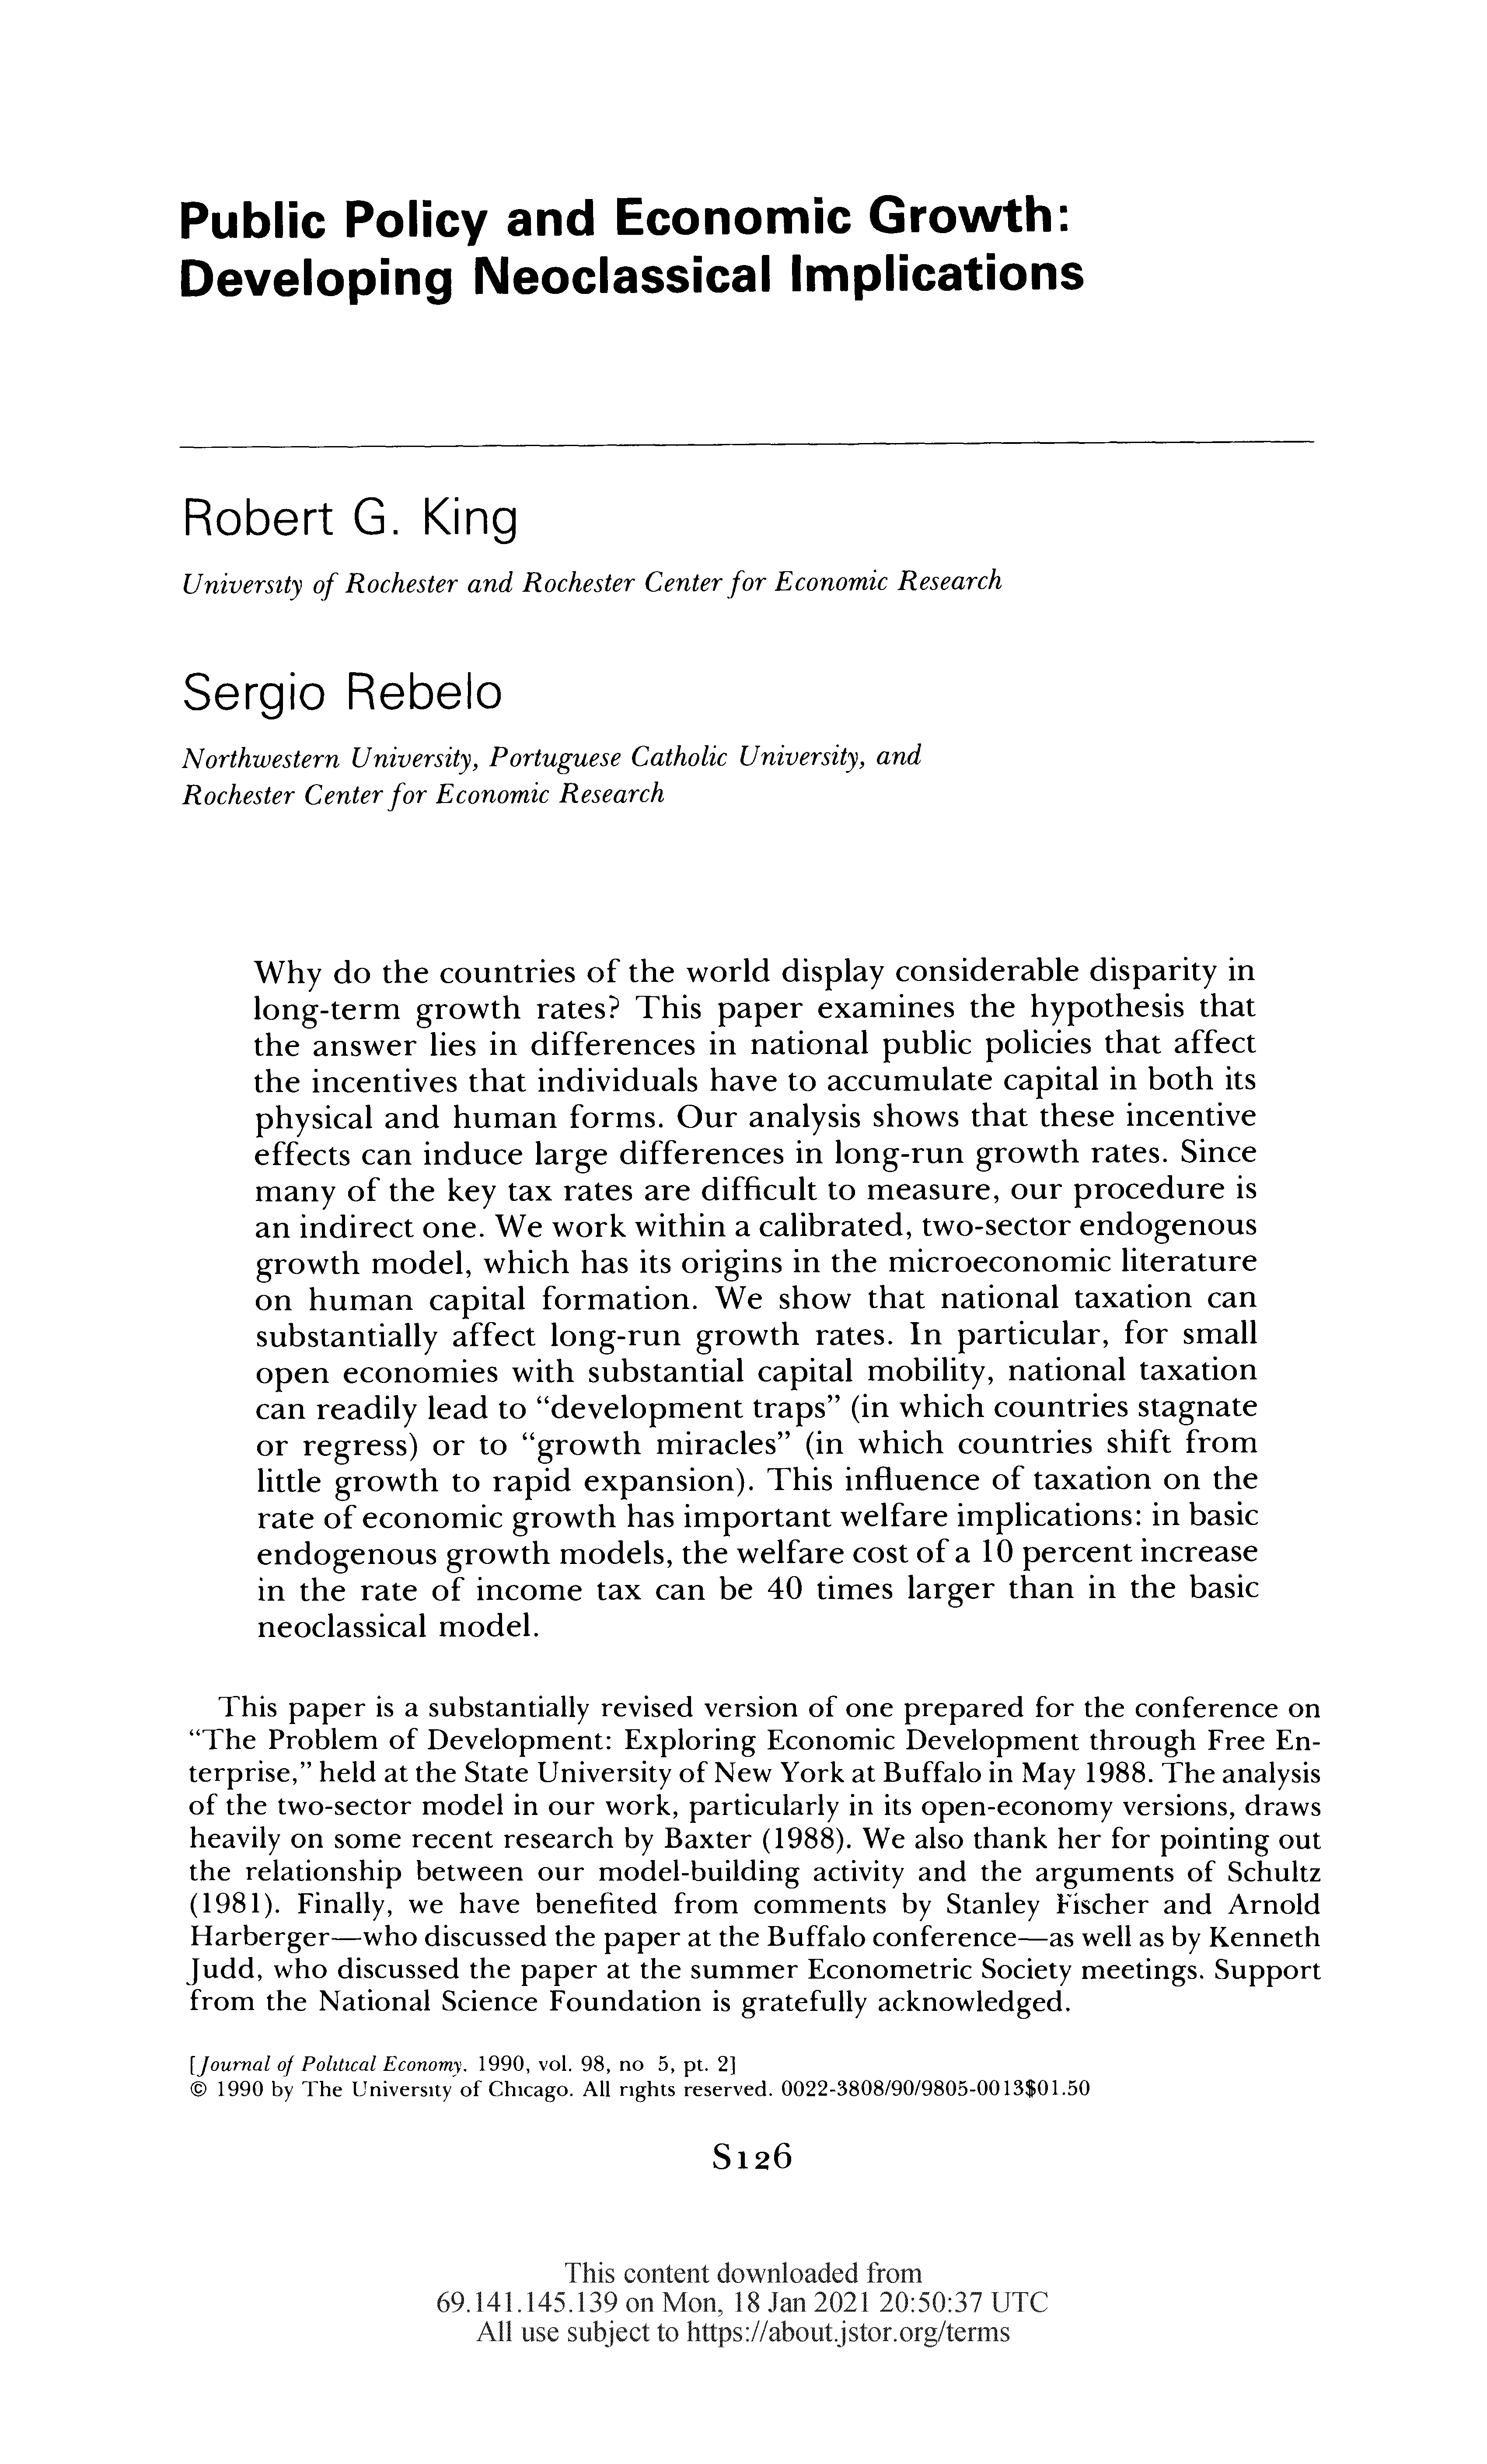
\includegraphics[width=0.8\linewidth]{king.png}
			\end{column}
			\begin{column}{0.56\textwidth}
				\begin{center}
					\textit{\textcolor{blue}{Question:}}\\ \pause
					\bigskip		
					Why do the countries of the world display considerable disparity in long-term growth rates?\\ \pause
					\bigskip		
					What is the linkage between national policies and long-term rates of economic growth?
				\end{center}
			\end{column}
		\end{columns}
	\end{frame}
	
	\begin{frame}[fragile]{Theory}
		What is the neoclassical economic model?\pause
		\begin{itemize}
			\item Assumes a rational individual.
			\item Emphasize free-market and private property.\pause
			\item \textit{Equilibrium}: Where the supply and demand meet.\pause
			\begin{itemize}
				\item Market will find the optimal point--equilibrium by itself.
				\item Under the equilibrium, supply and demand are harmonious.\\Also, economies will show stable growth.
				\item Do not touch the market, government...! $\rightarrow$ Small Govt.
			\end{itemize}
		\end{itemize}
	\end{frame}
	
	\begin{frame}[fragile]{Theory}
		Existing explanations; neoclassical model
		\begin{itemize}
			\item See \citet[S129-S133]{king:rebelo:1990}. \pause
			\item Basic neoclassical model: \pause $Y_t = F(K_{t}, NX_{t})$ \pause
			\begin{itemize}
				\item $Y_t$: A single good in given time of $t$.
				\item $K_{t}$: Physical capital
				\item $NX_{t}$: Labor \pause
				\begin{itemize}
					\item $N$: Labor population
					\item $X_t$ Technological progress
				\end{itemize}
			\end{itemize}
		\end{itemize}
	\end{frame}
	
	\begin{frame}[fragile]{Theory}
		Existing explanations; neoclassical model
		\begin{itemize}
			\item See \citet[S129-S133]{king:rebelo:1990}.
			\item Basic neoclassical model: $Y_t = F(K_{t}, NX_{t})$ \pause $\rightarrow$ Let us translate it. \pause
			\begin{equation*}
				\begin{aligned}
					\text{Output(=Good)}_{t}&=F(\text{Physical capital}_{\text{(e.g. factory)}}\\ 
					&\times\:\text{Labor}_{\text{(=Labors and their skills)}})
				\end{aligned}
			\end{equation*} \pause
			\item Argues that population growth ($N$) and technology progress($X_t$) have exogenous effect on economic growth in the long-run. \pause
			\begin{itemize}
				\item Neoclassical model tells that public policies have only 'short-term' effect on economic growth. $\rightarrow$ Really?
			\end{itemize}
		\end{itemize}
	\end{frame}
	
	\begin{frame}[fragile]{Theory}
		\citet{king:rebelo:1990}
		\begin{itemize}
			\item Public policies can have long-term effect on economic growth.
			\item Economic growth = $F$(Changes in public policies)
		\end{itemize}
	\end{frame}
	
	\begin{frame}[fragile]{Theory}
		\citet{king:rebelo:1990}
		\begin{itemize}
			\item Public policies $\rightarrow$ Individuals' incentives\\$\rightarrow$ Levels of accumulation in physical and human capitals.
			\begin{itemize}
				\item Explore the effect of public policies on economic growth with two sectors; physical capital and human capital.
				\item Using the data from previous studies, \citet{king:rebelo:1990} replicate the results of neoclassical model and expand them into models under different settings.\pause
				\begin{itemize}
					\item Basic model (Only $N$ and $X_t$ matter)
					\item Simple endogenous growth model (Only consider the endogenous effect of economic growth on physical capitals) \item Two-sector endogenous growth model (Physical and human capitals)
				\end{itemize}
			\end{itemize}
		\end{itemize}
	\end{frame}
	
	\begin{frame}[fragile]{Findings}
		\begin{itemize}
			\item Public policies, especially national taxation, can substantially affect long-run growth rates. \pause
			\item Taxation may affect the growth rate in an important way, but that the magnitude of the influence depends on the production and tax structure. \pause
			\item Economic growth $\rightarrow$ Inequality in human capitals $\downarrow$ $\rightarrow$Economic growth. \pause
			\item Endogenous relationship
		\end{itemize}
	\end{frame}
	
	\section{Duflo. 2012.}
	\subsection{Women Empowerment and Economic Development}
	\begin{frame}[fragile]{General question}
		\begin{columns}[T]
			\begin{column}{0.4\textwidth}
				\includegraphics[width=0.8\linewidth]{duflo.png}
			\end{column}
			\begin{column}{0.56\textwidth}
				\begin{center}
					\textit{\textcolor{blue}{Question:}}\\ \pause
					\bigskip		
					Can economic development cause women's empowerment?\\ \pause
					\bigskip		
					Can economic development solve gender inequality?\\ \pause
					\bigskip
					Can women's empowerment cause economic development?
				\end{center}
			\end{column}
		\end{columns}
	\end{frame}
	
	\begin{frame}[fragile]{Theory}
		Existing studies on women empowerment and economic development \pause
		\begin{enumerate}
			\item Economic development $\uparrow$ $\rightarrow$ Gender inequality $\downarrow$ \pause
			\item Women empowerment $\uparrow$ (Gender inequality $\downarrow$)\\$\rightarrow$ Economic development $\uparrow$ \pause
		\end{enumerate}
		"This paper reviews the evidence on both sides of the empowerment-development relationship." \citep[1053]{duflo:2012} \pause
		\begin{itemize}
			\item When poverty is reduced, the condition of everyone, including women, improves. \pause
			\item Gender inequality declines as poverty declines, so the condition
			of women improves more than that of men with development.
		\end{itemize}
	\end{frame}
	
	\begin{frame}[fragile]{Theory}
		\begin{enumerate}
			\item Economic development $\uparrow$ $\rightarrow$ Gender inequality $\downarrow$  \pause
			\begin{itemize}
				\item Relaxing the grip of poverty (inequality $\downarrow$)
				\item Improving maternal mortality\\(=lower parental investment in childhood)
				\item Providing women hope by expanding their opportunities
				\item Freeing up women's time
			\end{itemize}
		\end{enumerate}
	\end{frame}
	
	\begin{frame}[fragile]{Theory}
		\begin{enumerate}
			\setcounter{enumi}{1}
			\item Gender inequality $\downarrow$ $\rightarrow$ Economic development $\uparrow$ \pause
			\begin{itemize}
				\item A woman's education, earnings, or political participation\\ $\rightarrow$ Family outcomes
				\item Giving women the right to vote makes a difference.
				\item Policies increasing women's welfare\\ $\rightarrow$ Costs of childcare $\downarrow$/women's access to the labor market$\uparrow$\\ $\rightarrow$ Economic development $\uparrow$
			\end{itemize}
		\end{enumerate}
		\bigskip \pause
		\citet{duflo:2012} utilizes literature survey and case studies.
		\begin{itemize}
			\item Literature on women's empowerment and development.
		\end{itemize}
	\end{frame}
	
	\begin{frame}[fragile]{Findings}
		\begin{itemize}
			\item Economic development can contribute to women's empowerment.\pause
			\begin{itemize}
				\item Also, women's empowerment can enhance economic development.\pause
				\item However, their magnitudes of relationship are not so great as previous literature argues.\pause
			\end{itemize}
			\item \textbf{Economic development is not a sole determinant for women's empowerment and vice versa.}\pause
			\item Policies targeted toward women can have immediate consequences.
		\end{itemize}
	\end{frame}
	
	\section{Summaries \& Questions}
	\begin{frame}[fragile]{Summaries}
		\begin{enumerate}
			\item \citet{king:rebelo:1990} \pause
			\begin{itemize}
				\item Public policies enhancing human capital can have positive effect on economic growth.
				\item However, is the budget always equal to the actual expenditure? \pause
				\begin{itemize}
					\item If not, there might be another factor that can affect public policies' effects on economic growth or even makes the effect biased. \pause
				\end{itemize} 
			\end{itemize}
			\item \citet{duflo:2012} \pause
			\begin{itemize}
				\item Previous studies report that women's empowerment and development have endogenous relationship. \pause
				\item However, `economic` development is not only the factor affects women empowerment. \pause
				\begin{itemize}
					\item Here, \citet{duflo:2012} suggests policies are necessary to improve gender inequality.
				\end{itemize}
			\end{itemize}
		\end{enumerate}
	\end{frame}
	
	\begin{frame}[fragile]{Summaries}
		\begin{itemize}
			\item \citet{king:rebelo:1990} and \citet{duflo:2012} have several implications. \pause
			\begin{itemize}
				\item Economic development, inequality, and poverty are intertwined.
				\begin{itemize}
					\item Need to be cautious to understand the causal relationship. \pause
				\end{itemize}
				\item Inequality and poverty are multidimensional.
				\begin{itemize}
					\item \citet{king:rebelo:1990} see this issue with respect to physical AND human capitals.
					\item \citet{duflo:2012} addresses it with various paths (household environment, political rights etc). \pause
				\end{itemize}
			\end{itemize}
			\item Even the topic of `development,` politics/policies matter.
		\end{itemize}
	\end{frame}
	
	\begin{frame}[fragile, c]{Questions}
		\begin{center}
			{\huge Thank you!}\\
			\bigskip		
			Any questions or meetings?\\
		\end{center}
		\begin{equation*}
			\begin{aligned}
				\text{\ding{43}}& \text{Email: \href{sp23@email.sc.edu}{sp23@email.sc.edu}}\\
				\text{\ding{43}}& \text{Calendly: \href{https://calendly.com/sanghoon}{\texttt{Here}}}
			\end{aligned}
		\end{equation*}
	\end{frame}
	
	\begin{frame}[t, fragile, allowframebreaks]{}
		\bibliographystyle{apsr}
		\bibliography{RD5.bib}
	\end{frame}
\end{document}
